\documentclass[aspectratio=169]{beamer}
\usepackage{estilo-presentacion}
\usetikzlibrary{matrix,backgrounds}

% ---------- Tablas húngaras (mismo dibujo que el documento) ----------
\tikzset{
  htab/.style={matrix of nodes, ampersand replacement=\&, row sep=0pt, column sep=0pt,
    nodes={text width=#1, align=center, minimum height=5.4mm, inner sep=1pt, font=\small, anchor=center},
    column 1/.style={nodes={text width=15mm, font=\small\bfseries}},
    row 1/.style={nodes={font=\scriptsize\bfseries}}},
  htab/.default=8mm,
  tapa/.style={line width=3pt, gray!60, line cap=round},
  asignado/.style={draw, circle, thick, minimum size=5mm, inner sep=0pt},
}
\newcommand{\rejilla}[3]{%
  \foreach \i in {2,...,#2}{\foreach \j in {2,...,#3}{%
    \draw[gray!55, thin] (#1-\i-\j.north west) rectangle (#1-\i-\j.south east);}}%
  \draw[thick] (#1-2-2.north west) rectangle (#1-#2-#3.south east);}
\newcommand{\sfila}[3]{\begin{pgfonlayer}{background}\fill[gray!16] (#1-#2-2.north west) rectangle (#1-#2-#3.south east);\end{pgfonlayer}}
\newcommand{\scol}[3]{\begin{pgfonlayer}{background}\fill[gray!16] (#1-2-#2.north west) rectangle (#1-#3-#2.south east);\end{pgfonlayer}}
\newcommand{\lfila}[3]{\begin{pgfonlayer}{background}\draw[tapa] ($(#1-#2-2.west)+(-4pt,0)$) -- ($(#1-#2-#3.east)+(4pt,0)$);\end{pgfonlayer}}
\newcommand{\lcol}[3]{\begin{pgfonlayer}{background}\draw[tapa] ($(#1-2-#2.north)+(0,4pt)$) -- ($(#1-#3-#2.south)+(0,-4pt)$);\end{pgfonlayer}}
\newcommand{\cero}[2]{\node[asignado] at (#1-#2) {};}
\newcommand{\pie}[4]{\node[font=\scriptsize\itshape, below=1mm, align=center] at ($(#1-#2-2.south west)!0.5!(#1-#2-#3.south east)$) {#4};}

\title{Casos particulares del problema de asignación}
\subtitle{Cuando la tabla no es ``perfecta''}
\author{Investigación de Operaciones · Asignación y flujo en redes}
\date{}

\begin{document}

% ---------------------------------------------------------------------
\begin{frame}
  \titlepage
\end{frame}

% ---------------------------------------------------------------------
\begin{frame}{Integrantes}
  \vspace{1em}
  \begin{enumerate}\setlength{\itemsep}{1.2em}
    \item \rule{0.7\textwidth}{0.4pt}
    \item \rule{0.7\textwidth}{0.4pt}
    \item \rule{0.7\textwidth}{0.4pt}
    \item \rule{0.7\textwidth}{0.4pt}
    \item \rule{0.7\textwidth}{0.4pt}
  \end{enumerate}
\end{frame}

% ---------------------------------------------------------------------
\begin{frame}{¿Qué son los casos particulares?}
  \begin{columns}[T]
    \begin{column}{0.5\textwidth}
      El método húngaro solo sabe resolver una tabla \textbf{cuadrada}, de \textbf{costos} a \textbf{minimizar},
      donde \textbf{todos pueden hacer todo}.

      \medskip
      \begin{block}{Ejemplo cotidiano}
        3 amigos, \textbf{4} tareas de la casa. Luis \textbf{no puede} hacer las compras, Ana puede hacer
        \textbf{dos} tareas, y si fueran puntos de gusto querríamos el \textbf{máximo}.
      \end{block}
    \end{column}
    \begin{column}{0.47\textwidth}
      \textbf{La idea:} no hace falta otro método.
      \begin{enumerate}
        \item \textbf{Preparar} la tabla.
        \item Aplicar el \textbf{húngaro} de siempre:\\
              {\small restar mínimos de filas y columnas, tapar ceros con el menor número de líneas,
              ajustar con $k$, asignar.}
        \item \textbf{Traducir} el resultado al problema real.
      \end{enumerate}
    \end{column}
  \end{columns}
\end{frame}

% ---------------------------------------------------------------------
\begin{frame}{Caso 1: problema no balanceado}
  \begin{columns}[c]
    \begin{column}{0.45\textwidth}
      \textbf{Receta:} si faltan agentes o tareas, agregar filas o columnas \textbf{ficticias} con costo \textbf{0}.

      \medskip
      Lo que le toque a lo ficticio \textbf{queda sin pareja}.

      \medskip
      {\small Ejemplo: 2 personas, 3 tareas. T3 le toca al ficticio: nadie la hace. Costo $4 + 3 = 7$.}
    \end{column}
    \begin{column}{0.5\textwidth}
      \centering
      \begin{tikzpicture}
        \matrix (a) [htab=9mm] {
         \& T1 \& T2 \& T3 \\
        Ana  \& 4 \& 6 \& 5 \\
        Beto \& 7 \& 3 \& 8 \\
        Ficticio \& 0 \& 0 \& 0 \\
        };
        \sfila{a}{4}{4}\rejilla{a}{4}{4}
        \cero{a}{2-2}\cero{a}{3-3}\cero{a}{4-4}
        \pie{a}{4}{4}{lo sombreado es ficticio}
      \end{tikzpicture}
    \end{column}
  \end{columns}
\end{frame}

% ---------------------------------------------------------------------
\begin{frame}{Caso 2: maximización}
  \begin{columns}[c]
    \begin{column}{0.34\textwidth}
      \textbf{Receta:} restar cada valor del \textbf{mayor} de la tabla.
      \[ \text{pérdida} = \text{mayor} - \text{valor} \]
      Minimizar lo que se deja de ganar $=$ ganar lo máximo.

      \medskip
      {\small Al final se suman las \textbf{ganancias originales}: $8 + 9 + 6 = 23$.}
    \end{column}
    \begin{column}{0.64\textwidth}
      \centering
      \begin{tikzpicture}
        \matrix (g) [htab=7mm, column 1/.style={nodes={text width=11mm, font=\small\bfseries}}] {
         \& T1 \& T2 \& T3 \\
        Ana  \& 8 \& 6 \& 3 \\
        Beto \& 5 \& 9 \& 4 \\
        Caro \& 7 \& 2 \& 6 \\
        };
        \rejilla{g}{4}{4}\pie{g}{4}{4}{ganancias}
      \end{tikzpicture}\quad
      \begin{tikzpicture}
        \matrix (h) [htab=7mm, column 1/.style={nodes={text width=11mm, font=\small\bfseries}}] {
         \& T1 \& T2 \& T3 \\
        Ana  \& 1 \& 3 \& 6 \\
        Beto \& 4 \& 0 \& 5 \\
        Caro \& 2 \& 7 \& 3 \\
        };
        \rejilla{h}{4}{4}\cero{h}{2-2}\cero{h}{3-3}\cero{h}{4-4}
        \pie{h}{4}{4}{pérdida $= 9 -$ ganancia}
      \end{tikzpicture}
    \end{column}
  \end{columns}
\end{frame}

% ---------------------------------------------------------------------
\begin{frame}{Caso 3: asignaciones prohibidas}
  \begin{columns}[c]
    \begin{column}{0.5\textwidth}
      \textbf{Receta:} poner un costo \textbf{$M$} gigantesco en la pareja imposible.
      \begin{itemize}
        \item Al restar queda $M - 13$, $M - 810$\dots: nunca llega a cero.
        \item Si al final hay que usar una $M$: el problema es \textbf{infactible}.
      \end{itemize}
    \end{column}
    \begin{column}{0.46\textwidth}
      \centering
      \begin{tikzpicture}
        \matrix (p) [htab] {
         \& T1 \& T2 \& T3 \\
        Ana  \& 9 \& \textbf{M} \& 7 \\
        Beto \& 6 \& 4 \& 3 \\
        Caro \& 5 \& 8 \& 1 \\
        };
        \rejilla{p}{4}{4}\cero{p}{2-2}\cero{p}{3-3}\cero{p}{4-4}
        \pie{p}{4}{4}{Ana no puede hacer T2: costo $9 + 4 + 1 = 14$}
      \end{tikzpicture}
    \end{column}
  \end{columns}
\end{frame}

% ---------------------------------------------------------------------
\begin{frame}{Caso 4: un agente que hace varias tareas}
  \begin{columns}[c]
    \begin{column}{0.5\textwidth}
      \textbf{Receta:} \textbf{copiar su fila} una vez por cada tarea que pueda hacer.
      \begin{itemize}
        \item Cada copia es ``un turno'' del mismo agente.
        \item Al final se \textbf{juntan las copias}.
      \end{itemize}
      {\small Ana hace T2 y T3, Beto hace T1: $5 + 4 + 2 = 11$.}
    \end{column}
    \begin{column}{0.46\textwidth}
      \centering
      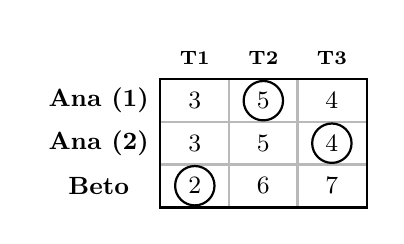
\begin{tikzpicture}
        \matrix (v) [htab] {
         \& T1 \& T2 \& T3 \\
        Ana (1) \& 3 \& 5 \& 4 \\
        Ana (2) \& 3 \& 5 \& 4 \\
        Beto    \& 2 \& 6 \& 7 \\
        };
        \rejilla{v}{4}{4}\cero{v}{2-3}\cero{v}{3-4}\cero{v}{4-2}
      \end{tikzpicture}
    \end{column}
  \end{columns}
\end{frame}

% ---------------------------------------------------------------------
\begin{frame}{Caso 5: óptimos múltiples}
  Al asignar hay \textbf{varias formas} de escoger un cero por fila y columna: \textbf{todas cuestan lo mismo}.
  \begin{center}
    \begin{tikzpicture}
      \matrix (x) [htab] {
       \& T1 \& T2 \& T3 \\
      Ana  \& 0 \& 0 \& 4 \\
      Beto \& 0 \& 0 \& 1 \\
      Caro \& 2 \& 5 \& 0 \\
      };
      \rejilla{x}{4}{4}\cero{x}{2-2}\cero{x}{3-3}\cero{x}{4-4}\pie{x}{4}{4}{opción A}
    \end{tikzpicture}\qquad\qquad
    \begin{tikzpicture}
      \matrix (y) [htab] {
       \& T1 \& T2 \& T3 \\
      Ana  \& 0 \& 0 \& 4 \\
      Beto \& 0 \& 0 \& 1 \\
      Caro \& 2 \& 5 \& 0 \\
      };
      \rejilla{y}{4}{4}\cero{y}{2-3}\cero{y}{3-2}\cero{y}{4-4}\pie{y}{4}{4}{opción B}
    \end{tikzpicture}
  \end{center}
  {\small Ojo: si solo se intercambian \textbf{copias del mismo agente}, es el mismo plan con otros nombres.
  Y si hay empates al tapar ceros, cualquier elección llega al mismo costo.}
\end{frame}

% ---------------------------------------------------------------------
\begin{frame}{Ejercicio: Job Shop Co. (Hillier y Lieberman)}
  {\small 3 máquinas, 4 ubicaciones, costo de manejo en \$/hora. La máquina 2 \textbf{no cabe} en la ubicación 2.}

  \medskip
  \centering
  \resizebox{\textwidth}{!}{%
  \begin{tikzpicture}
    \matrix (a) [htab] {
     \& U1 \& U2 \& U3 \& U4 \\
    Máq. 1 \& 13 \& 16 \& 12 \& 11 \\
    Máq. 2 \& 15 \& \textbf{M} \& 13 \& 20 \\
    Máq. 3 \& 5 \& 7 \& 10 \& 6 \\
    Ficticia \& 0 \& 0 \& 0 \& 0 \\
    };
    \sfila{a}{5}{5}\rejilla{a}{5}{5}\pie{a}{5}{5}{1. preparar: fila ficticia y $M$}
  \end{tikzpicture}
  \begin{tikzpicture}
    \node at (0,0) {$\Rightarrow$};
  \end{tikzpicture}
  \begin{tikzpicture}
    \matrix (b) [htab=10mm] {
     \& U1 \& U2 \& U3 \& U4 \\
    Máq. 1 \& 2 \& 5 \& 1 \& 0 \\
    Máq. 2 \& 2 \& $M{-}13$ \& 0 \& 7 \\
    Máq. 3 \& 0 \& 2 \& 5 \& 1 \\
    Ficticia \& 0 \& 0 \& 0 \& 0 \\
    };
    \sfila{b}{5}{5}\lfila{b}{2}{5}\lfila{b}{3}{5}\lfila{b}{4}{5}\lfila{b}{5}{5}\rejilla{b}{5}{5}
    \pie{b}{5}{5}{2. restar mínimos (11, 13, 5, 0)\\ 3. hacen falta 4 líneas: asignar}
  \end{tikzpicture}
  \begin{tikzpicture}
    \node at (0,0) {$\Rightarrow$};
  \end{tikzpicture}
  \begin{tikzpicture}
    \matrix (c) [htab=10mm] {
     \& U1 \& U2 \& U3 \& U4 \\
    Máq. 1 \& 2 \& 5 \& 1 \& 0 \\
    Máq. 2 \& 2 \& $M{-}13$ \& 0 \& 7 \\
    Máq. 3 \& 0 \& 2 \& 5 \& 1 \\
    Ficticia \& 0 \& 0 \& 0 \& 0 \\
    };
    \sfila{c}{5}{5}\rejilla{c}{5}{5}\cero{c}{2-5}\cero{c}{3-4}\cero{c}{4-2}\cero{c}{5-3}
    \pie{c}{5}{5}{4. asignación}
  \end{tikzpicture}}

  \bigskip
  \raggedright
  M1 $\to$ U4, \ M2 $\to$ U3, \ M3 $\to$ U1; la U2 queda vacía. \quad
  \res{Z^* = 11 + 13 + 5 = 29 \text{ \$/h}}
\end{frame}

% ---------------------------------------------------------------------
\begin{frame}{Ejercicio: vendedores y zonas (maximizar)}
  {\small Ejercicio adaptado, al estilo de Taha y de Anderson, Sweeney y Williams. Ventas en miles de \$/mes.}

  \medskip
  \begin{columns}[c]
    \begin{column}{0.33\textwidth}
      \centering
      \begin{tikzpicture}
        \matrix (v) [htab=7mm, column 1/.style={nodes={text width=11mm, font=\small\bfseries}}] {
         \& N \& S \& E \& O \\
        Ana   \& 44 \& 80 \& 52 \& 60 \\
        Beto  \& 60 \& 56 \& 40 \& 72 \\
        Carla \& 36 \& 60 \& 48 \& 48 \\
        Diego \& 52 \& 76 \& 36 \& 40 \\
        };
        \rejilla{v}{5}{5}\pie{v}{5}{5}{ventas; el mayor es 80}
      \end{tikzpicture}
    \end{column}
    \begin{column}{0.33\textwidth}
      \centering
      \begin{tikzpicture}
        \matrix (q) [htab=7mm, column 1/.style={nodes={text width=11mm, font=\small\bfseries}}] {
         \& N \& S \& E \& O \\
        Ana   \& 24 \& 0  \& 16 \& 20 \\
        Beto  \& 0  \& 16 \& 20 \& 0  \\
        Carla \& 12 \& 0  \& 0  \& 12 \\
        Diego \& 12 \& 0  \& 28 \& 36 \\
        };
        \lfila{q}{3}{5}\lfila{q}{4}{5}\lcol{q}{3}{5}\rejilla{q}{5}{5}
        \pie{q}{5}{5}{pérdida, filas y columnas:\\ 3 líneas $\Rightarrow$ ajuste $k = 12$}
      \end{tikzpicture}
    \end{column}
    \begin{column}{0.33\textwidth}
      \centering
      \begin{tikzpicture}
        \matrix (t) [htab=7mm, column 1/.style={nodes={text width=11mm, font=\small\bfseries}}] {
         \& N \& S \& E \& O \\
        Ana   \& 12 \& 0  \& 4  \& 8  \\
        Beto  \& 0  \& 28 \& 20 \& 0  \\
        Carla \& 12 \& 12 \& 0  \& 12 \\
        Diego \& 0  \& 0  \& 16 \& 24 \\
        };
        \rejilla{t}{5}{5}\cero{t}{2-3}\cero{t}{3-5}\cero{t}{4-4}\cero{t}{5-2}
        \pie{t}{5}{5}{4 líneas: asignar}
      \end{tikzpicture}
    \end{column}
  \end{columns}

  \bigskip
  Ana $\to$ Sur, Beto $\to$ Oeste, Carla $\to$ Este, Diego $\to$ Norte. \quad
  \res{Z^* = 80 + 72 + 48 + 52 = 252}
\end{frame}

% ---------------------------------------------------------------------
\begin{frame}{Ejercicio: Better Products Co. (Hillier y Lieberman)}
  \begin{columns}[c]
    \begin{column}{0.47\textwidth}
      {\small 3 plantas, 4 productos, costo diario en \$. Plantas 1 y 2 pueden hacer \textbf{dos} productos;
      la planta 2 \textbf{no puede} hacer el producto 3.}
      \begin{itemize}\small
        \item Copiar las filas de P1 y P2.
        \item 5 filas, 4 productos: columna ficticia.
        \item $M$ en (P2, producto 3).
        \item Dos ajustes con $k = 30$.
      \end{itemize}
      P1 $\to$ 2 y 3, \ P2 $\to$ 1, \ P3 $\to$ 4.\\[3pt]
      \res{Z^* = 3\,290 \text{ \$/día}}

      \smallskip
      {\scriptsize Óptimos múltiples: la otra asignación solo intercambia copias; es el mismo plan.}
    \end{column}
    \begin{column}{0.5\textwidth}
      \centering
      \resizebox{\linewidth}{!}{%
      \begin{tikzpicture}
        \matrix (w) [htab=11.5mm, column 1/.style={nodes={text width=17mm, font=\small\bfseries}}] {
         \& Prod.~1 \& Prod.~2 \& Prod.~3 \& Prod.~4 \& Ficticia \\
        P1 (1) \& 50 \& 0   \& 0  \& 90 \& 30 \\
        P1 (2) \& 50 \& 0   \& 0  \& 90 \& 30 \\
        P2 (1) \& 0  \& 30  \& $M{-}870$ \& 20 \& 0  \\
        P2 (2) \& 0  \& 30  \& $M{-}870$ \& 20 \& 0  \\
        P3     \& 0  \& 120 \& 0  \& 0  \& 60 \\
        };
        \scol{w}{6}{6}\rejilla{w}{6}{6}
        \cero{w}{2-3}\cero{w}{3-4}\cero{w}{4-2}\cero{w}{5-6}\cero{w}{6-5}
        \pie{w}{6}{6}{tabla final: 5 líneas, se asigna}
      \end{tikzpicture}}
    \end{column}
  \end{columns}
\end{frame}

% ---------------------------------------------------------------------
\begin{frame}{La calculadora}
  \begin{columns}[c]
    \begin{column}{0.5\textwidth}
      \centering
      \captura[0.72\textheight]{m9}\\[2pt]
      {\scriptsize Better Products Co. (memoria 9)}
    \end{column}
    \begin{column}{0.5\textwidth}
      \centering
      \captura[0.72\textheight]{m7}\\[2pt]
      {\scriptsize Job Shop Co. (memoria 7)}
    \end{column}
  \end{columns}
\end{frame}

% ---------------------------------------------------------------------
\begin{frame}{Conclusiones}
  \begin{itemize}\setlength{\itemsep}{0.5em}
    \item Los casos particulares \textbf{no necesitan otro método}: se prepara la tabla y se usa el húngaro.
    \item \textbf{No balanceado} $\to$ ficticios con 0. \quad \textbf{Máximo} $\to$ restar del mayor.
    \item \textbf{Prohibida} $\to$ costo $M$. \quad \textbf{Varias tareas} $\to$ copiar la fila.
    \item El total siempre se calcula con los \textbf{valores originales}.
    \item Óptimos múltiples: varias asignaciones con el mismo costo (¡revisar si no son solo copias!).
    \item Los tres ejercicios coinciden con la calculadora, el Simplex, la librería y la fuerza bruta: 29, 252 y 3\,290.
  \end{itemize}
\end{frame}

% ---------------------------------------------------------------------
\begin{frame}{Referencias}
  \small
  \begin{itemize}\setlength{\itemsep}{0.6em}
    \item Hillier, F. S. y Lieberman, G. J. \textit{Introducción a la Investigación de Operaciones}. McGraw-Hill.
          Capítulo de transporte y asignación.
    \item Taha, H. A. \textit{Investigación de Operaciones}. Pearson. Modelo de asignación.
    \item Anderson, D. R., Sweeney, D. J. y Williams, T. A. \textit{Métodos cuantitativos para los negocios}. Cengage.
    \item Winston, W. L. \textit{Investigación de Operaciones: aplicaciones y algoritmos}. Thomson.
    \item Kuhn, H. W. (1955). The Hungarian method for the assignment problem. \textit{Naval Research Logistics Quarterly}, 2.
  \end{itemize}
\end{frame}

\end{document}
